%# -*- coding: utf-8-unix -*-

\chapter{\LaTeX 排版用例}\label{chap:example}

本部分可参考SJTU Thesis模板\cite{SJTUThesis}的用例,源代码存放在tex文件夹下的examples.tex文件中,非常详尽。鄙人和其他开发者对其中几个部分有一些自己的见解,另外文献中也有一些没有提及的内容,写在本文档中。

\section{流程图}

对于不想花时间学习tizk宏包的同学,我们推荐在Power Point中绘制好流程图,然后导出pdf格式插入到文档中,学习成本较低,效果也非常好。

\section{表格}

SJTU Thesis中的表格介绍非常详尽,但其实有非常简单的从Excel生成\LaTeX 表格代码的方式,即Excel宏——excel2latex\footnote{\url{https://www.ctan.org/pkg/excel2latex?lang=en}}。此宏非常强大,可配合xcolor包生成有底色的表格。强烈推荐大家使用,提升撰写效率。

\begin{savenotes} % LaTeX通常不推荐在表格中插入脚注。但是,通过使用savenotes + makesavenoteenv 组合可在表格中插入脚注。请参考:https://en.wikibooks.org/wiki/LaTeX/Footnotes_and_Margin_Notes#Common_problems_and_workarounds

表\ref{tab:bicap}是github用户summershrimp提供的一个\textbf{双语标题}和\textbf{在标题中使用脚注}的示例,对标题有特殊需求的同学可以参考此处的源代码:
\begin{table}[H]
  \centering
  \bicaption[chinese]{一个颇为标准的三线表格\footnote{这个例子来自\href{http://www.ctan.org/tex-archive/macros/latex/contrib/booktabs/booktabs.pdf}{《Publication quality tables in LATEX》}(booktabs宏包的文档)。这也是一个在表格中使用脚注的例子,请留意与threeparttable实现的效果有何不同。}}[english]{A standard three-line table\footnote{该表格演示了如何使用bicaption插入双语标题}}
  \label{tab:bicap}
  \begin{tabular}{@{}llr@{}} \toprule
    \multicolumn{2}{c}{Item} \\ \cmidrule(r){1-2}
    Animal & Description & Price (\$)\\ \midrule
    Gnat & per gram & 13.65 \\
    & each & 0.01 \\
    Gnu & stuffed & 92.50 \\
    Emu & stuffed & 33.33 \\
    Armadillo & frozen & 8.99 \\ \bottomrule
  \end{tabular}
\end{table}

\end{savenotes}

\LaTeX 中表格的使用体验比Word差很多,很遗憾这是不可避免的。除了使用上文提到的excel2latex宏之外,可以在word中打好表格,然后截图插入论文也不失为一种方案。此外,在线表格转换工具\footnote{http://www.tablesgenerator.com}也不失为一种高效的excel表格至\LaTeX 的转换方案。

对于较长较大的表格,可以参考\LaTeX 笔记——lnotes2\footnote{\url{}http://dralpha.altervista.org/zh/tech/lnotes2.pdf}中的longtable(跨页表格)和sidewaystable(横向表格)等表格环境进行实现。另外可以使用\verb!p{2pt}!替代表格中的rcl,来控制表格每一列的宽度。

\section{图片表格指定位置插入}

图片和表格的插入默认是htbp四个选项,有时候这会让图片表格遍布整篇论文,可能会有同学非常反感这种情况,为了强制在当前位置插入图片,可以使用float宏包,然后使用H选项:\verb+\begin{figure}[H]+即可强制\TeX 在当前位置插入图片,从而避免正文和图片表格相距太远。

\section{多列图片}
由Github用户cvcore提供方案及示例代码,如需对两幅或多幅图片进行横向排版,建议使用subcaption包里的subfigure功能。效果如下:

\begin{figure}[H]
\centering
\begin{subfigure}{.45\textwidth}
  \centering
  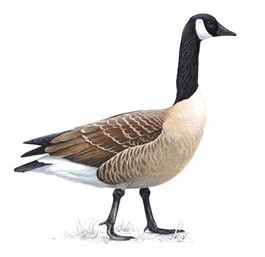
\includegraphics[width=.9\linewidth]{test.jpg}
  \caption{左图}
  \label{fig:test_subfigure1}
\end{subfigure}
\begin{subfigure}{.45\textwidth}
  \centering
  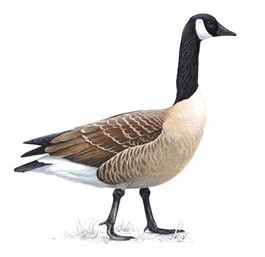
\includegraphics[width=.9\linewidth]{test.jpg}
  \caption{右图}
  \label{fig:test_subfigure2}
\end{subfigure}
\caption{这是一个并列子图}
\label{fig:test_subfigure}
\end{figure}

请注意每行subfigure宽度的总和尽量不要超过一个\textbackslash textwidth,否则图像会自动折叠至下一行。
